
\subsubsection{Pipeline}

En el proceso de integración del código de desarrollo a la versión de producción, \textit{Pull Request}, conforme al diseño realizado en la sección ~\nameref{par:testing}, se ejecuta el proceso denominado \textit{pipeline}.
Este proceso garantiza la entrega de software testeado y con el estándar de calidad requerido.
En la~\cref{fig:ci} se muestran los pasos de Integración Continua \textit{Continuous Integration} que se ejecutan cada vez que un desarrollador intenta comenzar un proceso de integración de código en fase de desarrollo a la rama de producción.
Mientras va programando, cada vez que sube código al repositorio se ejecutan los tests y la comprobación de calidad y seguridad, únicamente sobre el código nuevo.
Una vez es aprobado el código se procede a realizar los pasos de Entrega Continua \textit{Continuous Delivery} que se muestran en la~\cref{fig:cd}.
Este proceso incluye de nuevo la ejecución de los tests y la calidad, pero ya se ejecuta sobre todo el repositorio, actualizando las métricas globales de cobertura de tests y seguridad.
En total los procesos diferentes que se ejecutan se aprecian en la~\cref{fig:tasks}:

\begin{itemize}
    \item Ejecutar los tests.
    \item Chequeo de estándar del código o \textit{Code Style}.
    \item Compila la aplicación en modo producción, actualiza la rama principal del repositorio, actualiza la versión actual del sistema.
    \item Sube el código completo al servidor.
    En este proyecto este último paso está contemplado pero no desarrollado.
\end{itemize}

\begin{figure}[H]
    \centering
    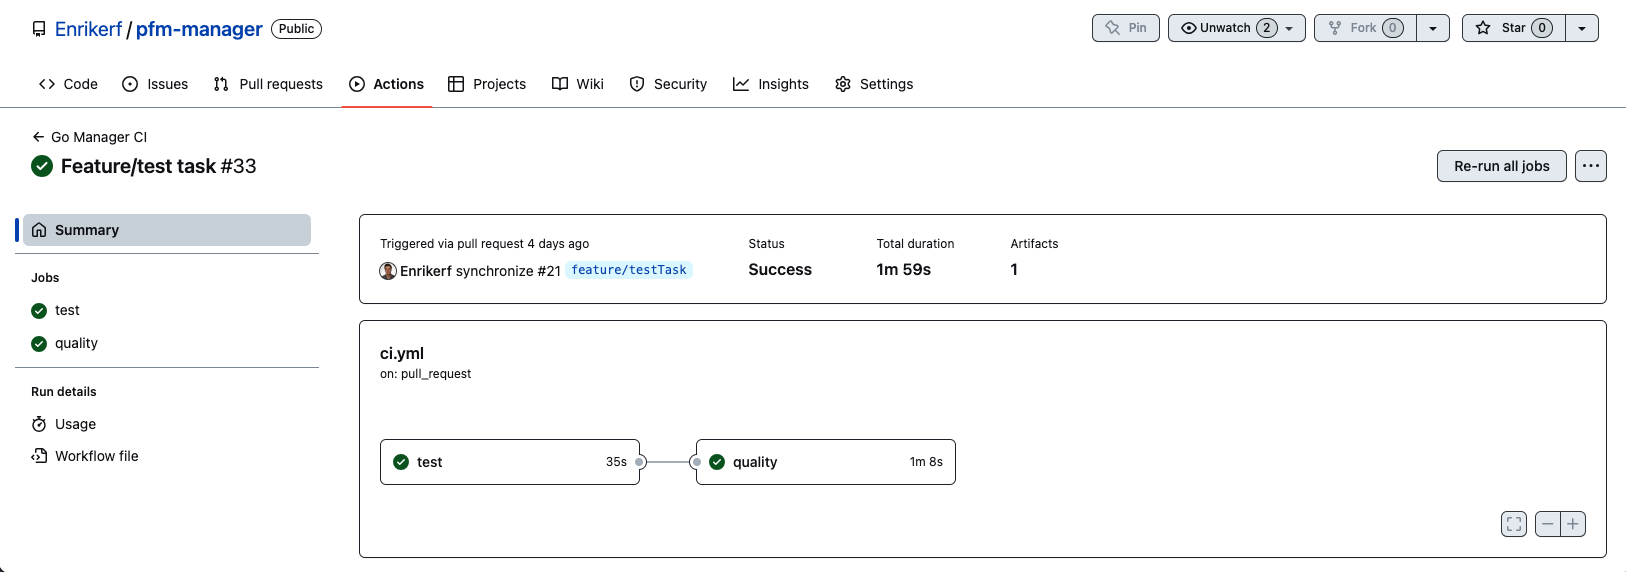
\includegraphics[height=0.23\textheight]{./part/Ejecucion/Seguimiento/PuestaAPunto/img/CI pipeline PR}
    \caption{Ejemplo de ejecución del Pipeline de integración continua, CI, en Github}\label{fig:ci}
\end{figure}

\begin{figure}[H]
    \centering
    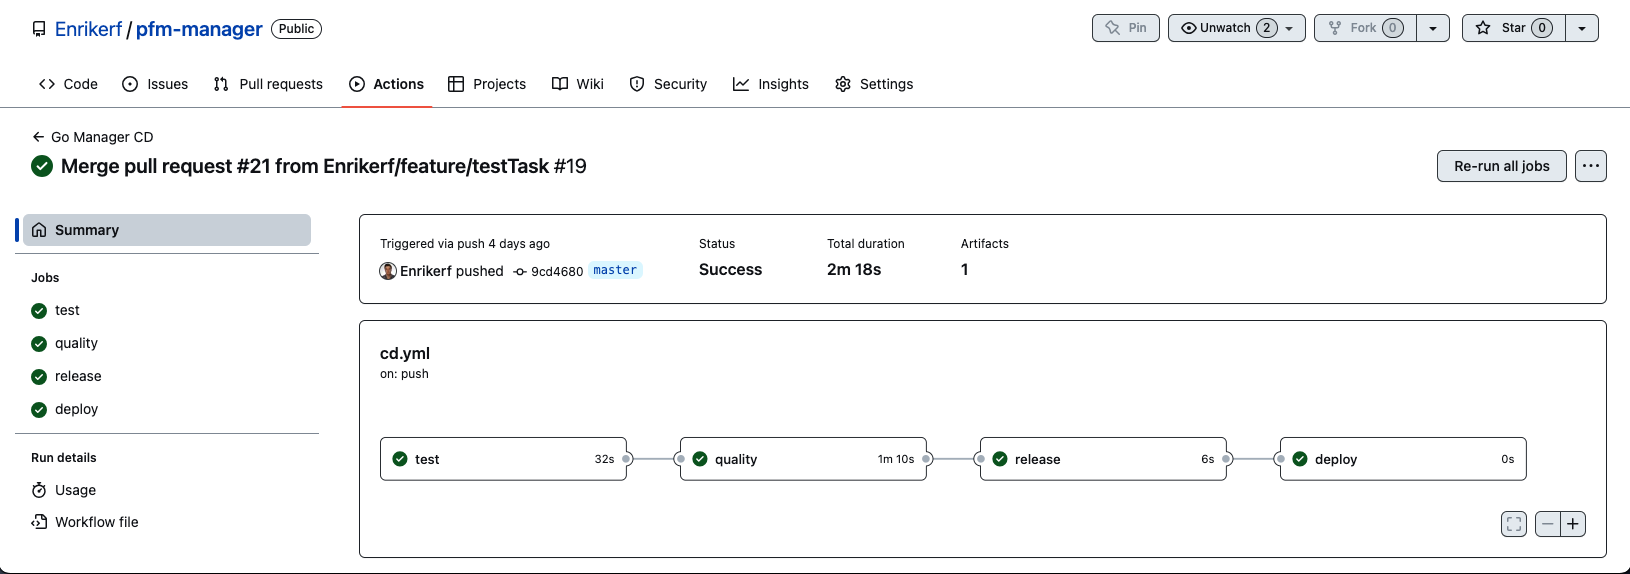
\includegraphics[height=0.23\textheight]{./part/Ejecucion/Seguimiento/PuestaAPunto/img/CD pipeline release}
    \caption{Ejemplo de ejecución del Pipeline de entrega continua, CD, en Github}\label{fig:cd}
\end{figure}

\begin{figure}[H]
    \centering
    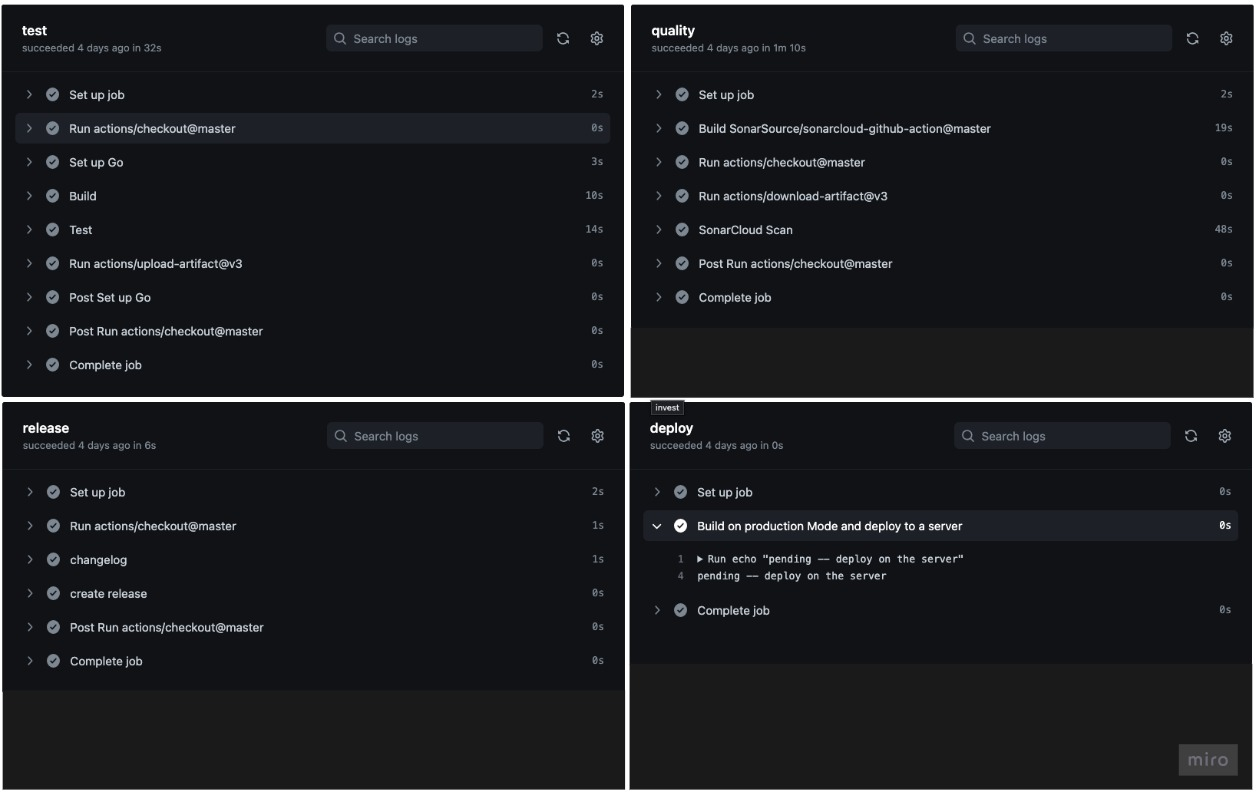
\includegraphics[height=0.43\textheight]{./part/Ejecucion/Seguimiento/PuestaAPunto/img/PFM - fullpipeline}
    \caption{Ejemplo de ejecución de Tareas CI/CD en Github}\label{fig:tasks}
\end{figure}

El proceso de comprobación de calidad se ejecuta con un sistema aparte.
Hay distintas soluciones de software comercial que ofrecen estas funcionalidades de comprobación y conteo de métricas de calidad.
En este proyecto se utiliza \href{https://sonarcloud.io/project/overview?id=Enrikerf_pfm-manager}{Sonarcloud}.
En cada subida de código al repositorio que está en un proceso de \textit{Pull Request} se ejecuta el análisis de métricas del código nuevo.
En la~\cref{fig:sonarcloudPR} se muestra un ejemplo donde se aprecia que en ese intento de integración se ha cubierto con tests el 100\% del código desarrollado.
Además de ofrecer comprobaciones de que no hay fallos conocidos de seguridad, como subidas de claves secretas.
No hay duplicidades que pudieran optimizarse y no hay bugs conocidos.

\begin{figure}[H]
    \centering
    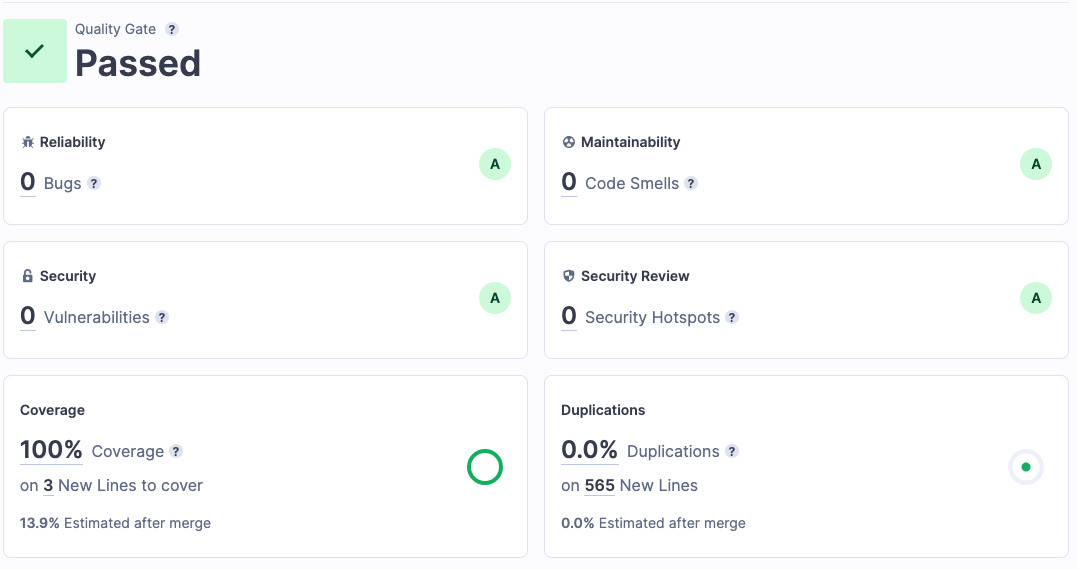
\includegraphics[height=0.35\textheight]{./part/Ejecucion/Seguimiento/PuestaAPunto/img/Sonarcloud Pr pipe}
    \caption{Ejemplo de métricas resultado de ejecución de Sonarcloud para una PR de Github}\label{fig:sonarcloudPR}
\end{figure}

\subsubsection{Montaje del hardware}

Para probar el sistema dispone de un montaje Hardware, cuyo diagrama conceptual se puede ver en  figura~\cref{fig:despliegue de prueba}.
Cuyo aspecto real se puede ver en la~\cref{fig:montaje en protoboard}.
Muestra el montaje físico de conexión entre el el servidor cliente y el dispositivo controlado.
El servidor Raspberry se conecta mediante \textit{protoboard} realizando la conexión con el puente H y el motor de corriente continua.

\begin{figure}[H]
    \centering
    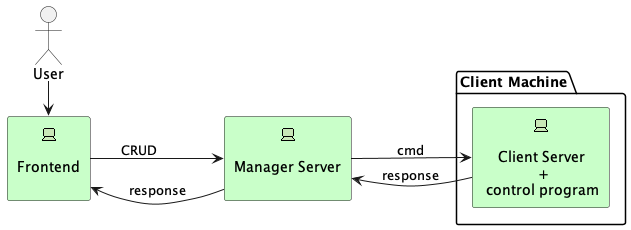
\includegraphics[height=0.2\textheight]{./part/Ejecucion/Seguimiento/PuestaAPunto/img/deploy}
    \caption{Diagrama de despliegue de prueba}\label{fig:despliegue de prueba}
\end{figure}

\begin{figure}[H]
    \centering
    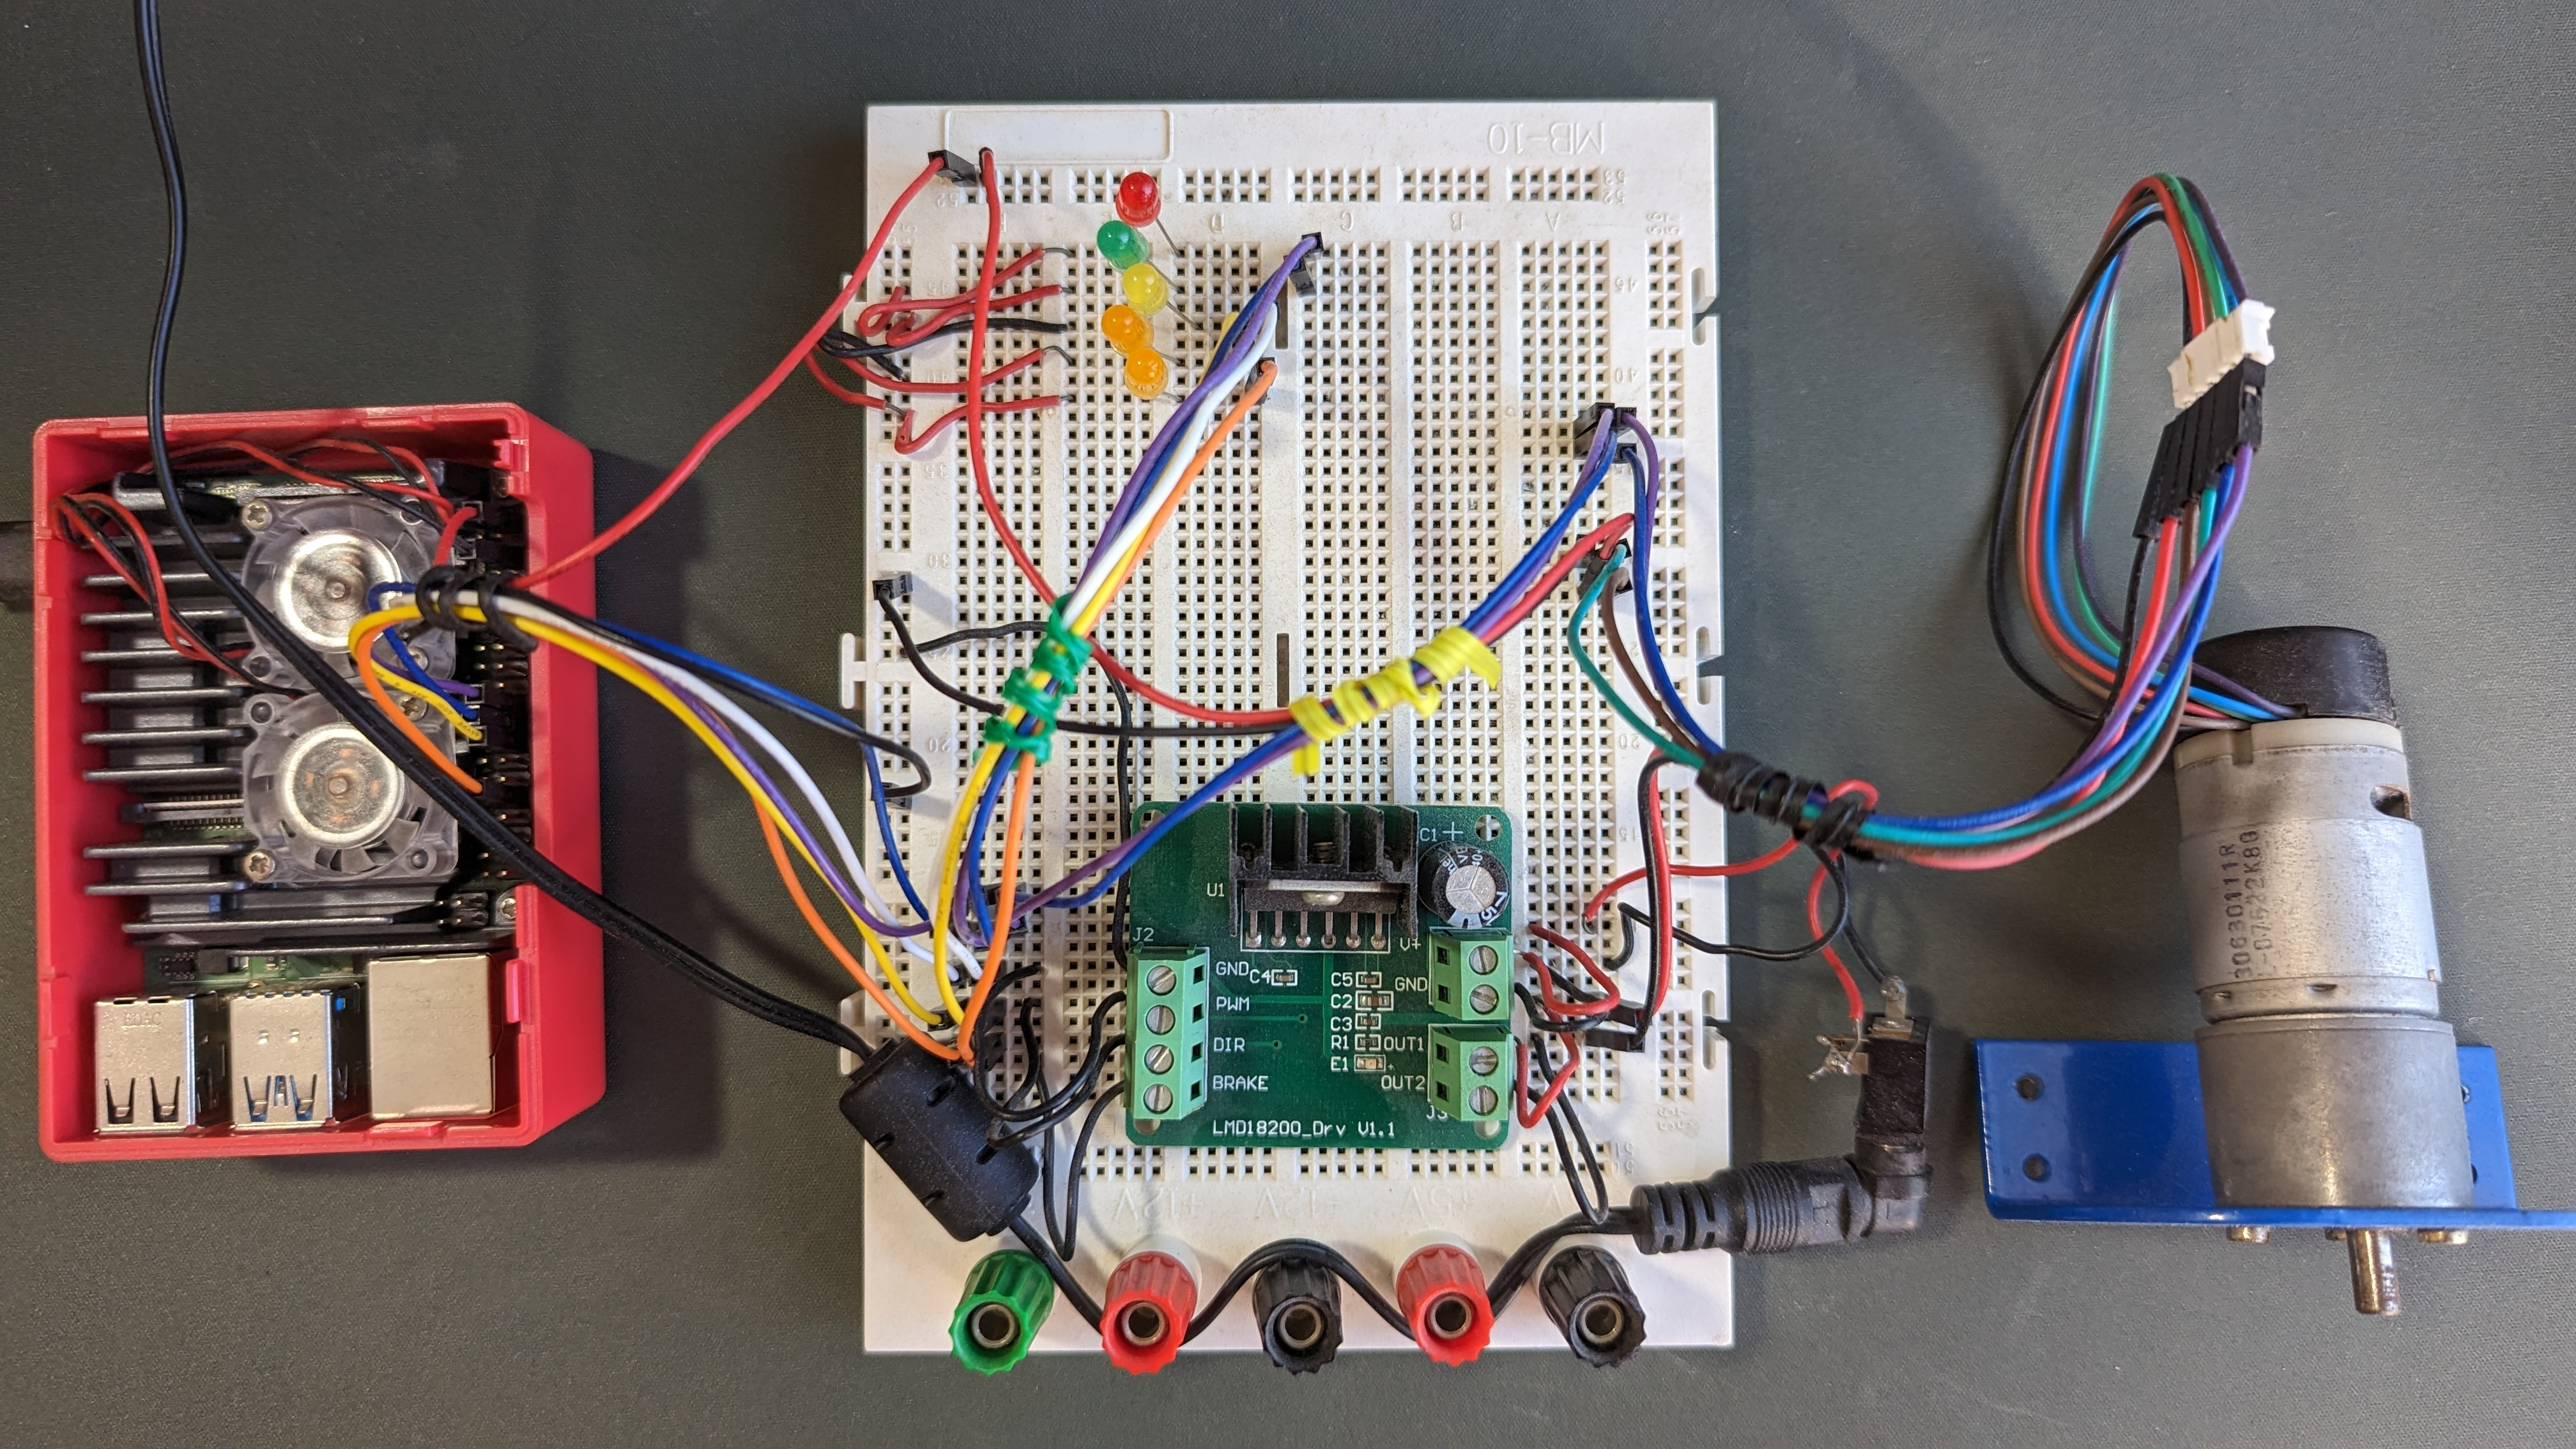
\includegraphics[height=0.35\textheight]{./part/Ejecucion/Seguimiento/PuestaAPunto/img/montajeProtoboard}
    \caption{Montaje en protoboard}\label{fig:montaje en protoboard}
\end{figure}

\subsubsection{Interfaz gráfica}

Para controlar el programa manager se ha desarrollado como añadido una interfaz gráfica.
No formaba parte de los objetivos del proyecto, pero se consideró que facilitaba el uso de la API disponible del programa Manager y la visualización de los resultados.
En la~\cref{fig:UITasks} se muestra el aspecto del listado de las tareas creadas en el sistema.
Permite visualizar el estado, la dirección en la que se encuentra el servidor cliente.
Se dispone también de un botón de acceso a la visualización de las ejecuciones pasadas de la tarea, es decir, los \textit{Batches}.
Desde la sección de los lotes de ejecución, o \textit{Batches}, se dispone un acceso a los resultados en plano;
o si son de tipo \textit{Stream} de datos numéricos se pueden mostrar en una gráfica.
Del mismo modo se dispone de un botón para ejecutar manualmente o volver a ejecutar las tareas automáticas.

Se considera interesante como linea futura mejorar esta interfaz para permitir todo el uso de la API: contemplar la creación, edición y borrado todos los elementos.
Uno de los puntos de investigación es arrojar claridad sobre el estado de la compatibilidad del flujo bidireccional con un navegador.
Si hay librerías experimentales lo suficientemente estables como para ser utilizadas con cierta garantías y que permítan extraer todos los beneficios de la comunicación gRPC\@.

\begin{figure}[H]
    \centering
    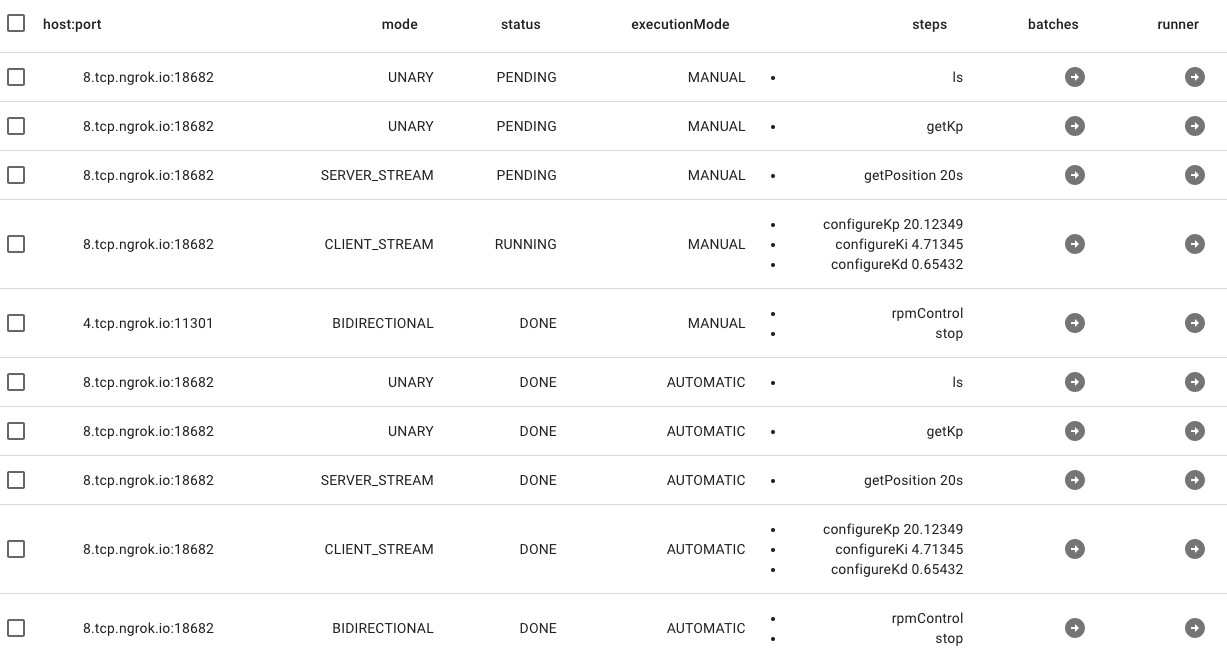
\includegraphics[height=0.35\textheight]{./part/Ejecucion/Seguimiento/PuestaAPunto/img/UItasks}
    \caption{Interfaz gráfica: listado de tareas}\label{fig:UITasks}
\end{figure}

\subsubsection{Resultados}

A lo largo de todo el documento se ha ido trabajando más en la garantía de calidad del código, los procesos y paradigmas utilizados que en un enfoque experimental.
Sin embargo las pruebas también han constado de una experimentación para poner a prueba los límites del sistema.
Se han puesto a prueba:
\begin{itemize}
    \item La calidad la gestión de la asincronía por parte del código y de Go.
    \item La estabilidad y versatilidad de los distintos tipos de comunicación implementados: unitario, \textit{stream} de cliente, \textit{stream} de servidor y bidireccional.
    \item La combinación de ambos factores en el control de velocidad PID del motor
\end{itemize}

\textbf{Experimento de velocidad mínima}

Se ha creado un comando en el programa cliente, ejecutable desde el manager, que va incrementando el ciclo de trabajo del PWM hasta que el encoder da una señal indicando que el motor ha empezado a moverse.
De esta forma además de probar la zona muerta experimentamos con la comunicación de tipo unitaria.
Con este experimento podemos, para cualquier motor, comprobar su zona muerta de forma remota.
En la Raspberry los pines PWM disponen de una resolución que va desde el 0 hasta el 16.777.216 para dividir el ciclo de trabajo entre 0 y 100\%.
La frecuencia utilizada es la máxima de la que dispone el sistema para estos pines que son 10 KHz.
Con estas premisas, para el motor utilizado la zona muerta se encuentra en el ciclo de trabajo equivalente a 1.258.292.

\textbf{Experimento de velocidad máxima}

De forma análoga se ha dispuesto de otro comando que permite establecer el ciclo de trabajo máximo y dando un margen de aceleración se devuelve al velocidad máxima alcanzada.
Para el motor utilizado esta velocidad máxima se encuentra en 200 RPM\@.
Como podemos ver en la~\cref{tab:EMG30specifications} esto se encuentra 16 RPM por debajo de las especificaciones para este dispositivo en concreto.

\textbf{Experimentos con la asincronía del encoder}

Utilizando únicamente el programa cliente, para mayor precisión, se dispuso el motor a girar a la velocidad mínima, para facilitar el conteo de vueltas.
Con el motor girando a un ciclo de trabajo constante y sin carga se ha contado los pulso del encoder recogidos durante 50 vueltas ofreciendo las 360 pulsaciones del encoder en cada una.
Después se ha probado ejecutando un programa en paralelo en el mismo sistema operativo de la Raspberry.
Dicho programa bloquea artificialmente la CPU lanzando procesos que únicamente esperan un tiempo determinado.
Monitorizando el sistema, y llegando a ocupar el 90\% de la CPU este proceso artificial, el conteo de pulsaciones del encoder se mantuvo en 360 por vuelta.

Un estudio más exhaustivo en este aspecto se considera una linea futura interesante.
Convendría mejorar la forma de establecer unas condiciones de experimentación que garanticen una doble comprobación del conteo de pulsos: el ofrecido por el encoder en el programa y una forma mecánica externa.
También establecer una monitorización no sólo de los recursos de la máquina si no el seguimiento de todos los hilos de ejecución y comprobar los bloqueos y esperas efectivas de cada hilo de ejecución.

\textbf{Experimento cualitativo de comunicaciones}

Para poner a prueba las latencias de comunicación ante un uso habitual en este tipo de sistemas se dispuso cada programa en una máquina y en una red separada.
De esta forma la comunicación se forzaba a ser externa a través de IP pública.
La comunicación se realizó sin ninguna modificación en el comportamiento apreciable.
Sin embargo, el principal resultado de este experimento es el descubrimiento de un concepto implementado por el lenguaje conocido como \textit{context}.
El contexto es un objeto implementado de forma nativa que guarda toda la información relativa a la ejecución y permite pasar el contexto de una función a otra para poder depurar mejor, sabiendo qué partes del código son llamadas por otras.

Aunque la trazabilidad a nivel de ejecución es de por sí un elemento valioso, que convendría implementar, su beneficio más importante se obtiene con las \textit{Gorutines}.
El contexto permite ser comunicado a cada una de las \textit{Gorutines} para darles conocimiento del tiempo de ejecución que están consumiendo dentro del sistema general que las ha generado.
Esto permite garantizar que ningún hilo de ejecución se quede huérfano.
A nivel de Infraestructura no disponemos de esa garantía y conforme pasa el programa tiempo en ejecución pueden darse comportamientos inesperados no controlados.

\textbf{Experimento de control PID}

Por último una prueba general del control de velocidad implementado, aunque no se ha llegado a una sintonización efectiva si se tomó este ejemplo de ejecución como un experimento general del sistema.
Se hace uso de la comunicación de \textit{streaming} del servidor tanto desde el manager a la interfaz gráfica como del programa cliente a el manager.
A la vez se hace uso de la asincronía al disponer de un comando separado en paralelo de tipo unitario para forzar la parada de dicho control.

En la~\cref{fig:UIRunner} se puede ver la evolución de la variable controlada, en radianes por segundo, para una consigna de 80rpm;
8.37758 rad/s equivalentes.

Los parámetro utilizados son:
\begin{itemize}
    \item Frecuencia del PWM 10 KHz.
    \item Tiempo de muestreo de 10ms.
    \item Ciclo de trabajo entre 1.258.292 y 16.777.216, de su rango de valores posibles.
\end{itemize}

Con estos parámetros se procede a una sintonización manual del PID hasta obtener una respuesta oscilante en torno a la consigna.
No se abarca mayor precisión en el sintonizado porque la conclusión principal de este experimento es que el sistema no dispone de una forma de guardar toda la precisión de la que nos provee el control y por lo tanto no se puede realizar una gráfica aceptable.
Los resultados se guardan con un tiempo de creación con precisión del segundo, el estándar en una base de datos, pero para el control necesitamos poder almacenar precisiones mayores.
Esto se puede apreciar en la figura~\cref{fig:UIRunner} donde la gráfica que se obtiene no contiene toda la resolución del control que efectivamente está ocurriendo.
En la base de datos se guardan varios puntos de resultado bajo el mismo segundo, imposibilitando el visionado correcto.


\begin{figure}[H]
    \centering
    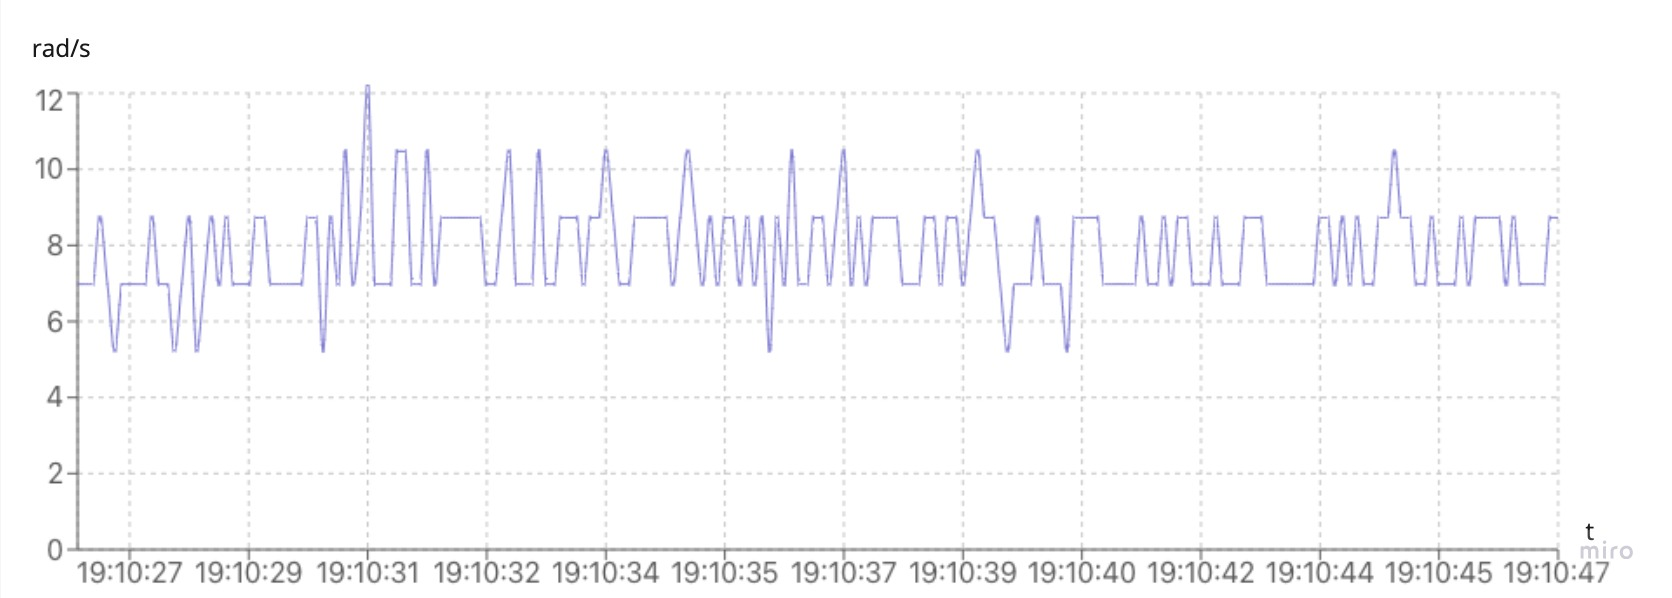
\includegraphics[height=0.2\textheight]{./part/Ejecucion/Seguimiento/PuestaAPunto/img/UIRunner}
    \caption{Interfaz gráfica: resultado ante ejecución manual de control en velocidad}\label{fig:UIRunner}
\end{figure}